% ****************************************************************************************** % Dissertation template and document class for Princeton University
% Author  : Jeffrey Scott Dwoskin <jdwoskin@princeton.edu>
% Adapted from: http://www.math.princeton.edu/graduate/tex/puthesis.html
% ****************************************************************************************** %


%%% For print copies
%% set 'singlespace' option to set entire thesis to single space, and define "\printmode" to remove all hyperlinks for printed copies of the thesis. Delete all output files before changing this mode -- it will turn hyperref package on and off
%\documentclass[12pt,lot, lof, singlespace]{puthesis}
%\newcommand{\printmode}{}

%%% For the electronic copy, use doublespacing, define "\proquestmode" to use outlined links, instead of colored links. 
\documentclass[12pt,lot, lof]{puthesis}
\newcommand{\proquestmode}{}
% I prefer proquestmode to be off for electronic copies for normal use, since the colored links are less distracting. However when printed in black and white, the colored links are difficult to read. 

%%% For early drafts without some of the frontmatter
% Also see the "ifodd" command below to disable more frontmatter
%\documentclass[12pt]{puthesis}

%%%%%%%%%%%%%%%%%%%%%%%%%%%%%%%%%%%%%%%%%%%%%%%%%%%%%%%%%%%%%\
%%%% Author & title page info

\title{Development of Photon Calibrator for Hardware Injection Test}

\submitted{June 2018}  % degree conferral date (January, April, June, September, or November)
\copyrightyear{2018}  % year in which the copyright is secured by publication of the dissertation.
\author{Yu-Kuang Chu}
\adviser{Wo-Lung Lee}  %replace with the full name of your adviser
%\departmentprefix{Program in}  % defaults to "Department of", but programs need to change this.
\department{Physics}

%%%%%%%%%%%%%%%%%%%%%%%%%%%%%%%%%%%%%%%%%%%%%%%%%%%%%%%%%%%%%\
%%%% Tweak float placements
% From: http://mintaka.sdsu.edu/GF/bibliog/latex/floats.html "Controlling LaTeX Floats"
% and based on: http://www.tex.ac.uk/cgi-bin/texfaq2html?label=floats
% LaTeX defaults listed at: http://people.cs.uu.nl/piet/floats/node1.html

% Alter some LaTeX defaults for better treatment of figures:
    % See p.105 of "TeX Unbound" for suggested values.
    % See pp. 199-200 of Lamport's "LaTeX" book for details.
    %   General parameters, for ALL pages:
    \renewcommand{\topfraction}{0.85}	% max fraction of floats at top
    \renewcommand{\bottomfraction}{0.6}	% max fraction of floats at bottom
    %   Parameters for TEXT pages (not float pages):
    \setcounter{topnumber}{2}
    \setcounter{bottomnumber}{2}
    \setcounter{totalnumber}{4}     % 2 may work better
    \setcounter{dbltopnumber}{2}    % for 2-column pages
    \renewcommand{\dbltopfraction}{0.66}	% fit big float above 2-col. text
    \renewcommand{\textfraction}{0.15}	% allow minimal text w. figs
    %   Parameters for FLOAT pages (not text pages):
    \renewcommand{\floatpagefraction}{0.66}	% require fuller float pages
	% N.B.: floatpagefraction MUST be less than topfraction !!
    \renewcommand{\dblfloatpagefraction}{0.66}	% require fuller float pages

% The documentclass already sets parameters to make a high penalty for widows and orphans. 

%%%%%%%%%%%%%%%%%%%%%%%%%%%%%%%%%%%%%%%%%%%%%%%%%%%%%%%%%%%%%\
%%%% Use packages

%\usepackage{amsfonts}

%%% For figures
\usepackage{graphicx}
%\usepackage{subfig,rotate}

%%% for comments
\usepackage{verbatim}

%%% For tables
\usepackage{multirow}
% Longtable lets you have tables that span multiple pages.
\usepackage{longtable}

% Booktabs produces far nicer tables than the standard LaTeX tables.
%   see: http://en.wikibooks.org/wiki/LaTeX/Tables
\usepackage{booktabs}

%set parameters for longtable:
% default caption width is 4in for longtable, but wider for normal tables
\setlength{\LTcapwidth}{\textwidth}


\usepackage{amsmath}


%%%%%%%%%%%%%%%%%%%%%%%%%%%%%%%%%%%%%%%%%%%%%%%%%%%%%%%%%%
%%% Printed vs. online formatting
\ifdefined\printmode

% Printed copy
% url package understands urls (with proper line-breaks) without hyperlinking them
\usepackage{url}


\else

\ifdefined\proquestmode
%ProQuest copy -- http://www.princeton.edu/~mudd/thesis/Submissionguide.pdf

% ProQuest requires a double spaced version (set previously). They will take an electronic copy, so we want links in the pdf, but also copies may be printed or made into microfilm in black and white, so we want outlined links instead of colored links.
\usepackage{hyperref}
\hypersetup{bookmarksnumbered}

% copy the already-set title and author to use in the pdf properties
\makeatletter
\hypersetup{pdftitle=\@title,pdfauthor=\@author}
\makeatother

\else
% Online copy

% adds internal linked references, pdf bookmarks, etc

% turn all references and citations into hyperlinks:
%  -- not for printed copies
% -- automatically includes url package
% options:
%   colorlinks makes links by coloring the text instead of putting a rectangle around the text.
\usepackage{hyperref}
\hypersetup{colorlinks,bookmarksnumbered}

% copy the already-set title and author to use in the pdf properties
\makeatletter
\hypersetup{pdftitle=\@title,pdfauthor=\@author}
\makeatother

% make the page number rather than the text be the link for ToC entries
%\hypersetup{linktocpage}
\fi % proquest or online formatting
\fi % printed or online formatting


%%%%%%%%%%%%%%%%%%%%%%%%%%%%%%%%%%%%%%%%%%%%%%%%%%%%%%%%%%%%%\
%%%% Define commands

% Define any custom commands that you want to use.
% For example, highlight notes for future edits to the thesis
%\newcommand{\todo}[1]{\textbf{\emph{TODO:}#1}}


% create an environment that will indent text
% see: http://latex.computersci.org/Reference/ListEnvironments
% 	\raggedright makes them left aligned instead of justified
\newenvironment{indenttext}{
    \begin{list}{}{ \itemsep 0in \itemindent 0in
    \labelsep 0in \labelwidth 0in
    \listparindent 0in
    \topsep 0in \partopsep 0in \parskip 0in \parsep 0in
    \leftmargin 1em \rightmargin 0in
    \raggedright
    }
    \item
  }
  {\end{list}}

% another environment that's an indented list, with no spaces between items -- if we want multiple items/lines. Useful in tables. Use \item inside the environment.
% 	\raggedright makes them left aligned instead of justified
\newenvironment{indentlist}{
    \begin{list}{}{ \itemsep 0in \itemindent 0in
    \labelsep 0in \labelwidth 0in
    \listparindent 0in
    \topsep 0in \partopsep 0in \parskip 0in \parsep 0in
    \leftmargin 1em \rightmargin 0in
    \raggedright
    }

  }
  {\end{list}}



%%%%%%%%%%%%%%%%%%%%%%%%%%%%%%%%%%%%%%%%%%%%%%%%%%%%%%%%%%%%%\
%%%% Front-matter

% For early drafts, you may want to disable some of the frontmatter. Simply change this to "\ifodd 1" to do so.
\ifodd 0
% front-matter disabled while writing chapters
\renewcommand{\maketitlepage}{}
\renewcommand*{\makecopyrightpage}{}
\renewcommand*{\makeabstract}{}

% you can just skip the \acknowledgements and \dedication commands to leave out these sections.

\else


\abstract{
% Abstract can be any length, but should be max 350 words for a Dissertation for ProQuest's print indicies (150 words for a Master's Thesis) or it will be truncated for those uses.
%Photon Calibrator (PCal) can be used as an actuator for injecting artificial test signal into the interferometer to investigate its response to astrophysical gravitational waves. In order to get better performance in high frequency regime, we are developing a new PCal with high power (20 Watt) laser for our KAGRA detector.
Photon calibrator (Pcal) is an independent device that can provide artificial input to an interferometric gravitational-wave detector by exerting the radiation pressure of its own laser on the test mass mirror in the interferometer. It not only can provide a fiducial length reference for calibration purpose but also can inject simulated gravitational waveforms to verify the response of the interferometer to the astrophysical gravitational waves, known as hardware injection test. 
Currently, the injection signals (Excitations) are produced by KAGRA Digital System(DGS). These signals change the intensity of PCal Laser by acousto-optic modulators (AOM) inside the transmitter module of PCal. However, if the output signal from the Digital System is noisy, it force AOM to modulate laser intensity according to such noisy control signal, resulting in noisy radiation force on the End Test Mirror (ETM). In this dissertation, we implemented and characterized an analog filter known as the \emph{De-Whitening filter}. We installed it between Digital System output and PCal to address the noise problem while keeping the accuracy of injected signals.




Key Words: Photon Calibrator, Hardware Injection Test, Gravitational Waves, KAGRA

%=================
%
%
%Nowadays, many gravitational wave events had been detected by ground-based laser interferometers. To achieve these results, properly calibrating these detectors thereby reconstructing the gravitational wave strain data is an indispensable work. 
%
%Photon calibrator (Pcal) is a independent device that can provide artificial input to the interferometer by exerting the radiation pressure of its own laser on the test mass mirror in the interferometer. It not only can provide a fiducial length reference for calibration purpose but also can inject simulated gravitational waveforms to verify the response of interferometer to the astrophysical gravitational waves. 
%
%In order to get better performance in high frequency regime, we are developing a new PCal with high power (20 Watt) laser for our Kamioka Gravitational wave detector (KAGRA). However, we found that the noise from the current control system may not meet the requirement of our KAGRA PCal. 
%
%In this dissertation, we try to implement and characterize an analog filter known as \emph{De-Whitening filter} to address the noise problem while keeping the accuracy of injected signals.

}

\acknowledgements{
%I would like to thank...
Wolung Lee, Sadakazu Haino, Takayuki Tomaru, Nobuyuki Kanda, Yuki Inoue, Takaaki Yokozawa, Takahiro Yamamoto, Darkhan Tuyenbayev, Chihiro Kozakai, Chih-Hsun Lin, Ming-Lee Chu
Bin-Hua Hsieh KEK(Emiko Kotaki, Ayako Hagiwara, Ayako Ueda)(Kunihiko Hasegawa, Tomohiro Yamada, Takaharu Shishido, Rishabh Bajpai,) KAGRA(Mihoko Okinaka, Rie Kikuchi)(Takafumi Ushiba, Koki Okutomi, Takahiro Miyamoto and Yutaro Enomoto)  ASIOP (Pei-Rong Tsai, Chia-Yi Lee)


%I would like to thank the Math department for providing the original documentclass file that this class is based upon. I would like to thank my parents, without whom my life would not be possible. I would also like to thank my advisor, my dissertation committee, and my research collaborators because every graduate student needs to do so. And finally, I thank the members of my research group, to whom I leave this template to save you some of the trouble I had to go through getting my dissertation to compile in \LaTeX{}.  
%
%Don't forget to ask your advisor if your work was sponsored by a grant that needs to be acknowledged in this section.  
}

\dedication{To my parents.}

\fi  % disable frontmatter


%%%%%%%%%%%%%%%%%%%%%%%%%%%%%%%%%%%%%%%%%%%%%%%%%%%%%%%%%%%%%\
%%%% Hide some chapters

%%% If you want to produce a pdf that includes only certain chapters, specify them with includeonly, in addition to including all chapters below.
%\includeonly{ch-intro/chapter-intro}
%%% You can also specify multiple chapters.
%\includeonly{ch-intro/chapter-intro,ch-usage/chapter-usage}
%\includeonly{chap1,chap2,chap3}


%%%%%%%%%%%%%%%%%%%%%%%%%%%%%%%%%%%%%%%%%%%%%%%%%%%%%%%%%%%%%
%%%% Notes:

% Footnotes should be placed after punctuation.\footnote{place here.}
% Generally, place citations before the period~\cite{anotherauthor}.
% The proper usage for i.e., and e.g., include commas ``(e.g., option A, option B)''

%%%%%%%%%%%%%%%%%%%%%%%%%%%%%%%%%%%%%%%%%%%%%%%%%%%%%%%%%%%%%
%%%% Import chapters

\begin{document}

\makefrontmatter


% If you've disabled frontmatter, you can insert the toc manually
%\tableofcontents\clearpage

% \include lets us split up the document (and each include starts a new page):
\chapter{Introduction} 

When you got a new camera, you probably will take a lot of testing photos before you start to use it seriously. Similarly, we would like to test our gravitational wave detector before we use it to see the Universe.

Hardware injection test is a process to verify the performance of interferometer by sending sample signals into interferometer. Ideally, we should prepare some real gravitational waves as test signals. But it is practically hard to generate large enough artificial gravitational waves that are detectable by current technology. 

Therefore, instead of generating gravitational waves, people mimic the effect of celestial gravitational waves by displacing the mirror according to the simulated gravitational waveforms, changing arm length correspondingly, , comparing the optical readout in the main interferometer, thereby checking the response of their interferometer. 

Among different ways to push those Test Mass Mirrors in the main interferometer, radiation pressure of external laser beams have been used because its simplicity and stability. A dedicated auxiliary laser system called Photon Calibrator(PCal) has been developed for this purpose. 

In this dissertation, I will briefly explain what is photon calibrator and how it works for calibration and hardware injection purposes. Then, I will discuss the noise problem from current signal generating system that is used to control PCal Laser intensity. Finally, a possible solution, Analog De-Whitening Filter, has been manufactured and tested with Photon Calibrator in Kamioka Gravitational Wave Detector (KAGRA). 
 

\section{Introduction to Gravitational Wave}
\subsection{What is gravitational wave}

In the General Theory of Relativity proposed by Albert Einstein in 1915, phenomena caused by gravity can be interpreted as results of curved spacetime. This is one of his important works after his `Happiest Thought', which recorded in his unpublished article ``Fundamental Ideas and Methods of the Theory of Relativity, Presented in Their Development"\cite{Einstein:happy}. Among different ways to curve our spacetime, which can be described by corresponding metric tensor fields, there exist wavelike solutions describing ripples of spacetime known as gravitational waves.

However, the physical reality of gravitational wave was not so clear to everyone in the early days, even to Einstein himself~\cite{Einstein:prl, Einstein:ongw}. The main problem is that there exist some gauge degree of freedom in the theory due to the arbitrariness of coordinate choices. We have to know whether the gravitational waves we found are just gauge waves (vibration of coordinate) or the wave can have some observable consequences. 

One of the most important observational evidence implying the existence of real gravitational waves is the Hulse-Taylor pulsar~\cite{HulseTaylor:discovery}. Taylor demonstrated that the change of pulsar rotation speed can be explained by emission of gravitational wave~\cite{HulseTaylor:gr, HulseTaylor:gr2}.  

% in 2015 September 14th
Finally, on September 14th, 2015, the first direct detection of gravitational wave signal~\cite{gw:150914_det} is done by Laser Interferometer Gravitational-Wave Observatory(LIGO) detectors in the United States.

\subsection{How to describe gravitational wave}

In Einstein's General Relativity, gravitational effects are realized by geometry of spacetime. According to a great mathematician Bernhard Riemann, we can describe the geometry of certain space by telling the ``distance" between nearby points in the space. Practically, the information of distance between nearby spacetime points form a tensor called metric, which means the measure of distance. By choosing a coordinate system, one can write down those corresponding components of metric tensor $g$.
\begin{equation}
    g_{\mu\nu}=
\left(
\begin{array}{cccc}
  g_{00} & g_{01} & g_{02} & g_{03} \\
  g_{10} & g_{11} & g_{12} & g_{13} \\
  g_{20} & g_{21} & g_{22} & g_{23} \\
  g_{30} & g_{31} & g_{32} & g_{33}
\end{array}
\right)  
\end{equation}
 Now, we can calculate spacetime distance $ds$ between two nearby points by their coordinate separation:

\begin{equation}
    ds^2 = g_{\mu\nu} dx^{\mu} dx^{\nu}
\end{equation}




\begin{figure}[hbt!]
\centering
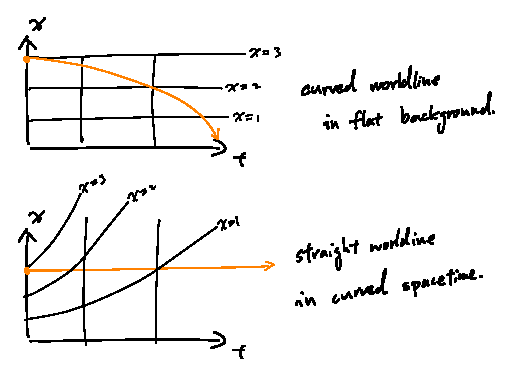
\includegraphics[width=0.8\textwidth]{figure/gr/curvedxt.eps}
\caption{Newtonian versus Einstein's point of view. }\label{fig:grxt}
\index{figures}
\end{figure}


Through the interaction between matter and spacetime, matter can curve our Universe. The whole story can be resolved by solving Einstein equation,
\begin{equation}
\label{eq:einsteineq}
    R_{\mu\nu}-\frac{1}{2}g_{\mu\nu}R = \frac{8 \pi G}{c^4} T_{\mu\nu}
\end{equation}
which is a non-linear differential equation of metric tensor field $g_{\mu\nu}(x^{\alpha})$ since the Ricci tensor $R_{\mu\nu}$ contains metric tensor and its differential.

It's similar to the case in Electrodynamics, in which we can have electromagnetic waves solutions by solving Maxwell equations in vacuum, that we can have gravitation wave solutions by solving vacuum Einstein equation. The situation will become even clear if we linearize the Einstein equation and choose coordinate or gauge properly.

%Gravitational phenomenon can be thought as the interaction between matter(Energy-Stress Tensor field) and the spacetime(Metric Tensor filed). This is similar to the case in Electrodynamics, in which the interaction between electrical charges and electrical/magnetic fields give us EM phenomenon. The mathematical formulae that govern EM phenomenon are Maxwell equations. 
% Given the the spacetime filled with metric tensor field which tell us the shape or geometry of our universe. 
 
 Let's start from 





\begin{equation}
    \Box \bar{h}_{\mu\nu} = - \frac{16\pi G}{c^4}T_{\mu\nu}
\end{equation}


%When it comes to gravitational wave, there is a very convenient gauge(coordinate) constrain called Traceless and Transverse gauge. 


the corresponding coordinates are attached to a set of free falling objects. 
for perturbation of wave like part metic over Schwarzschild background which represent Earth’s gravity.


Refer to \cite{maggiore:gw1}



How to generate gravitational wave
The source of electromagnetic wave is time-dependent electrical charge distribution.  Similarly, the source of gravitational wave is time-dependent mass(energy) distribution. Strictly speaking, the lowest order of mass multi-pole which can generate real gravitational waves is mass quadruple because we don’t have negative mass, while the electromagnet wave can be generate though time-dependent electrical dipole moment. The gravitational wave strain generated by mass quadruple can be approximately described by famous quadrupole formula:
(quadrupole formula)
Practically, PN NR....
According to our current understand of universe, there are several kinds of astrophysical gravitational wave sources, whose h(t) amplitude is large enough to be detected by current ground based laser interferometer, like advanced-LIGO, advanced-Virgo or KAGRA. 
Compact Binary Coalescence 
BNS BBH
\subsection{How to detect Gravitational wave}
The interaction of detector and gravitational wave can have different interpretation due to different coordinate choice\cite{ifo:gauge}. It is quiet similar to that the magnetic force in one observational frame may be electric force in the other frame. However, practically, I would like to use the …….., which described in next section.


\section{Detection of Gravitation wave}

Interaction of GW wave when $\lambda_gw$ L of detector
Limit of Michelson IFO
IFO with dual-recycling and Fabry-Perot  arms.
 Complex response
WE NEED Calibration Calibration Calibration



\section{Calibration and Reconstruction}

Calibration is always the fist step before we measure something by some device.
For example, to measure the weight of an apple, you should calibrate your scale by putting a “standard kilogram” on it. Then, you can either adjust the scale readout to be 1kg, or record the difference showed in scale readout, which may be used to reconstruct real weight of the apple. However, the spring constant of springs inside the scale could fluctuate due to temperature changes. To accurately measure the weight of the apple, we have to measure the calibration factor (scale readout when we put the standard mass on it.) when we measure the weight of apple, if possible, simultaneously.

Due to the complexity of practical interferometer, the response of interferometer itself to external gravitational source is not only sophisticated but also time-dependent. In reality, we “inject several calibration lines”, which means we displace the End-Test-Mirror by several known frequency and amplitude sine waves. Then, we try to see these standard signals in the readout of interferometer, thereby solving the response of interferometer.

\subsection{Transfer function of Laser Interferometer with Fabry-Perot Cavity}


\subsection{Tracking Time-dependent Response by Calibration lines}



\section{Photon Calibrator (Pcal)}
\subsection{Principle of Photon Calibrator}
Photon calibrator is an additional laser with high precision intensity modulator. It is installed in front of End-Test-Mass Mirror(ETM) and can push the ETM by radiation force due to its own Laser beam as depicted in Fig.(XX). To generate any artificial h(t) by Pcal, we have to translate desired h(t) into corresponding force F(t) exerting on ETM. This can be done by using equation of motion of the ETM suspend by its suspension system. Then, we control the Pcal Laser output intensity P(t) such that the radiation force exerted on ETM is F(t) we calculated before. 

The radiation force caused by a continuous laser beam can be calculated by its momentum transfer per unit time.

\begin{equation}
    \mathbf{F} = \frac{\Delta \mathbf{p}}{\Delta t}
\end{equation}
For our purpose, the laser beam will be almost reflected from ETM. Therefore, the momentum transfer to ETM per unit time should be almost equal to twice of longitudinal momentum flux carried by PCal laser beam.

\begin{equation}
\label{eq:f2cos}
    \mathbf{F}_\text{on ETM} = \frac{\Delta \mathbf{p}_\text{ETM}}{\Delta t}
    = 2 \cos(\theta) \frac{\Delta p_\text{Laser} }{\Delta t}
\end{equation}
where $\theta$ is the angle of incident.

Furthermore, one can express the momentum flux of light in terms of its intensity through Eq.(\ref{eq:epc}), which can be derived from either classical point of view with its Poynting vector or Quantum Mechanical approaches that we adopt here by dealing with photons. 

\begin{align}
   E_{\gamma} &= \hbar \omega \\
   p_{\gamma} &= \hbar k \\
              &= \frac{k}{\omega} ~ E_{\gamma} = \frac{1}{c}E_{\gamma}
\end{align}

\begin{align}
\label{eq:epc}
   \underbrace{\frac{\Delta p_{\text{photons}}}{\Delta t}}_{\text{momentum flux due to }\atop \text{photons in a continuous laser beam}}
   &= \frac{1}{c}
   \underbrace{ \frac{\Delta E_{\text{photons}}}{\Delta t} }_{\text{Intensity of laser beam}\atop \text{defined as } P}
   = \frac{P}{c} 
\end{align}

%\begin{align}
%    E_{\gamma} &= \hbar \omega \\
%    p_{\gamma} &= \hbar k \\
%               &= \frac{k}{\omega} ~ E_{\gamma} = \frac{1}{c}E_{\gamma}   \\
%    \frac{\Delta p_{\text{photons}}}{\Delta t}
%    &= \frac{1}{c} \frac{\Delta E_{\text{photons}}}{\Delta t} 
%    = \frac{P}{c} 
%\end{align}
Combining Eq.(\ref{eq:f2cos}) and Eq.(\ref{eq:epc}), the force that PCcal can give ETM is:

\begin{equation}
\label{eq:pcalforce}
    F_\text{PCal}(t) = \frac{ 2 \cos(\theta) }{c} P(t) 
\end{equation}


On the other hand, the equation of motion of suspend ETM can be modeled as:

\begin{equation}
\label{eq:etmeom}
    \ddot{x}(t) + b \dot{x}(t) + \omega_0^2 x(t) = \frac{F(t)}{M} 
%    F_\text{PCal}(t) = \frac{ 2 \cos(\theta) }{c} P(t) 
\end{equation}

%The solution to Eq.(\ref{eq:etmeom}) can be wrote as the combination of homogeneous part and particular solution:
%
%\begin{equation}
%%\label{eq:etmeom}
%    x(t)=x_h(t)+x_p(t)
%\end{equation}


The impulse response is

\begin{equation}
%\label{eq:etmeom}
    x(t)=\frac{b}{\omega_1}e^{-\frac{b}{2}(t-t_0)}\sin[\omega_1 (t-t_0)]
\end{equation}


And the transfer function is

\begin{equation}
\label{eq:etmtf}
   x(\omega)=\frac{-1}{\omega^2 - \omega_0^2 + i \omega b}F(\omega)
\end{equation}

As long as $\omega^2 \gg \omega_0^2$ and $\omega \gg b$, Eq.(\ref{eq:etmtf}) can be approximated as

\begin{equation}
%\label{eq:etmtf}
   x(\omega)=\frac{-1}{\omega^2}F(\omega)
\end{equation}

By substituting the Fourier transformed Eq.({\ref{eq:pcalforce}}) into it, we can get the expression of x(f) introduced by P(f)
\begin{equation}
\label{eq:pcaldisp}
    x(\omega) = \frac{-1}{M \omega} \frac{2  P(f) \cos(\theta)}{c} 
\end{equation}



\subsection{Evolution of Photon Calibrator}

Original Pcal is proposed by Glasgow group \cite{pcal:clubley2001}. They use single laser beam hitting on the center of ETM and successfully see these sin waves in the the readout of their interferometer. Later on, GEO...

 is that it may introduce drumhead mode vibration of ETM surface (just like the vibration mode you see when you hit the center of a drum), which introduce unwanted h(t) effectively. This problem is solved by LIGO group\cite{pcal:karki2016}, who separate the Pcal laser beam into two beams, hitting on the nodal point of drumhead mode on the ETM surface\cite{pcal:Daveloza2012}.  


In order to excite same amplitude h(t) in higher frequency regime, we have to give much larger F(t) since the relationship between x(t) and F(t) in an pendulum ……………….



\subsection{Why do we need Photon Calibrator}
\subsection{Tracking Time-dependent Response by Calibration lines}


\chapter{Hardware Injection through Photon Calibrator}
\section{Principle}



 
 As I described in Sec.\ref{sec:pcalth}, we can generate desired ETM displacement $x(t)$ by changing PCal laser intensity $P(t)$. One can calculate corresponding $P(t)$ by performing inverse Fourier transform to Eq.(\ref{eq:pcaldisp}).
 
\begin{align}
    \int_{-\infty}^{-\infty} x(\omega) e^{i \omega t} ~\mathrm{d} \omega &= 
     \frac{-2   \cos(\theta)}{Mc} 
     \int_{-\infty}^{-\infty}\frac{P(\omega)}{\omega^2} e^{i \omega t} ~\mathrm{d} \omega \\
\label{eq:pcaldispt}
    \frac{Mc}{-2 \cos(\theta)} \int_{-\infty}^{-\infty}
     x(\omega) \omega^2 e^{i \omega t} ~\mathrm{d} \omega 
&= P(t) 
\end{align}

where
\begin{align*}
%\label{eq:pcaleq}
   \text{Mass of ETM} \qquad  M &= 23 ~\mathrm{kg} \\
   \text{Arm Length} \qquad   L &= 3 ~\mathrm{km}  \\
   \text{Angle of Incident} \qquad   \theta &= 0.72 ~\mathrm{deg}  \\
   \text{Speed of Light} \qquad   c &= 2.998\times10^8 ~\mathrm{m/s} \\
\end{align*}
Also, if we have complete suspension model of ETM, we can substitute the $\omega^2$ factor in Eq.(\ref{eq:pcaldispt}) by the full displacement-to-force transfer function.


\pagebreak
\section{Experimental Setup}

Once we got the necessary P(t) from the desired x(t) through Eq.(\ref{eq:pcaldispt}), we can start to modulate our PCal laser intensity according to that P(t). The way how we control our PCal laser intensity is explained in Fig.~(\ref{fig:injsigpath}).


\begin{figure}[hbt!]
\centering
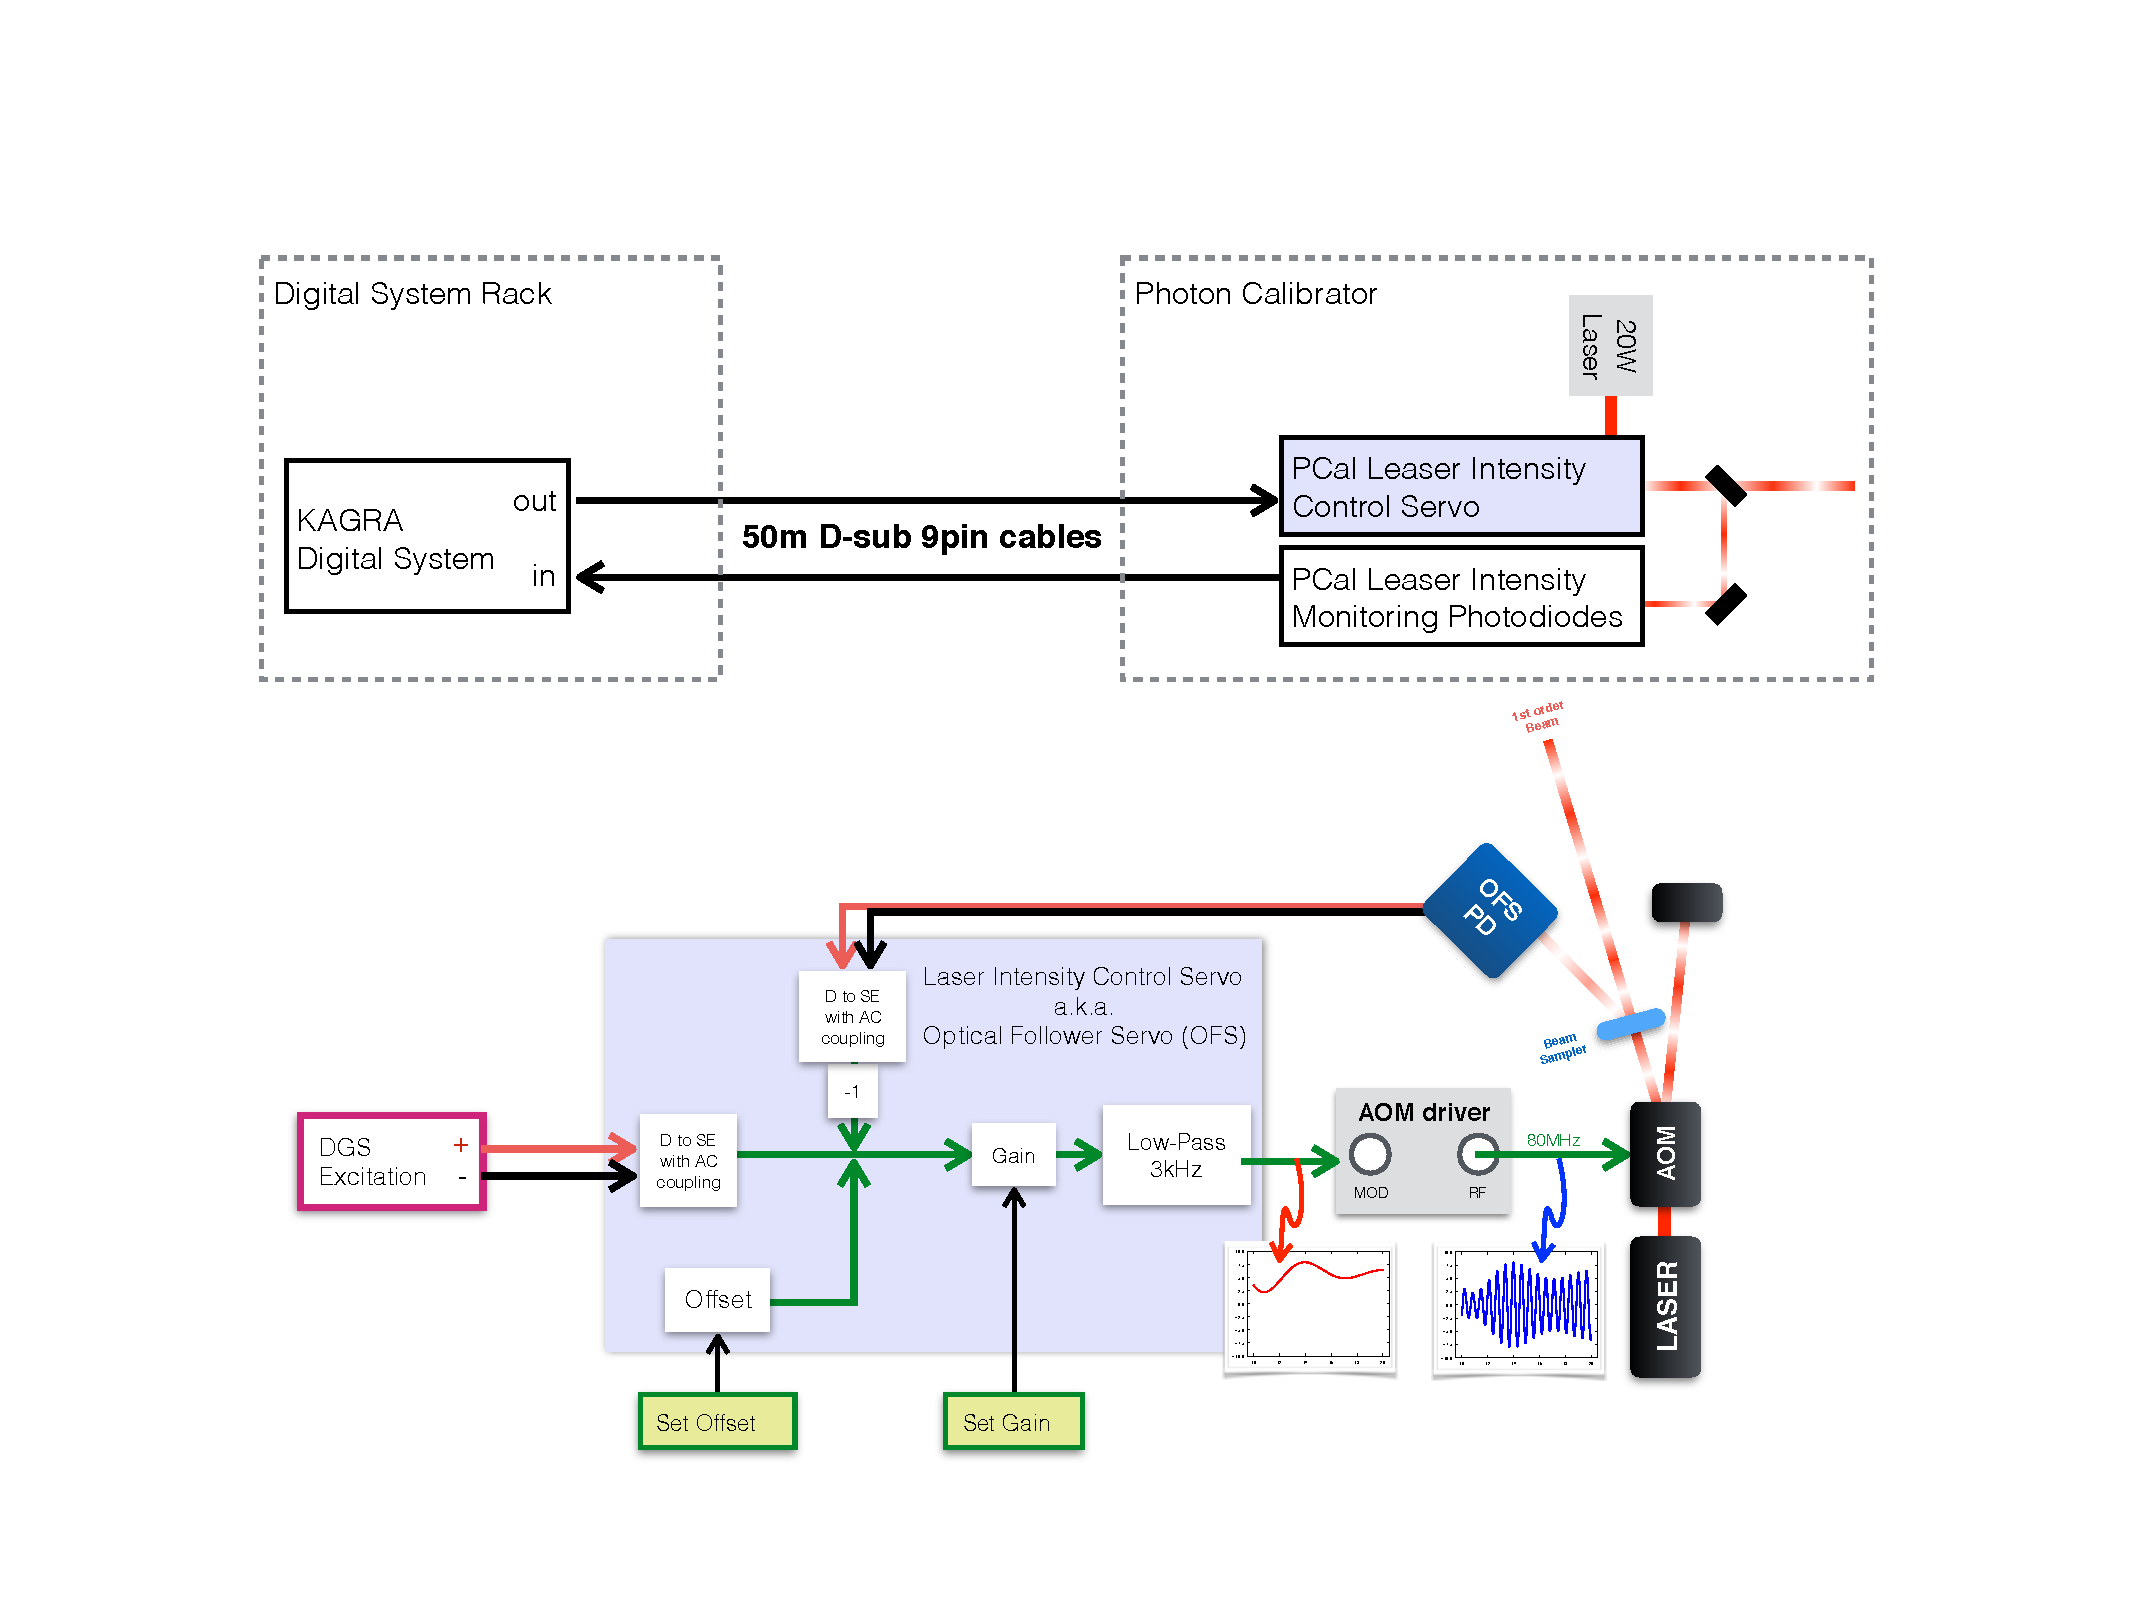
\includegraphics[width=1\textwidth]{figure/injsigpath}
\caption[Controlling PCal with Digital Control System]{Controlling PCal with Digital Control System. The PCal laser beam that will be sent to ETM is the first order diffracted beam of a 20W input laser form an acousto-optic modulator(AOM). Its intensity is controlled by the control signal from our KAGRA Digital System. An analog feedback control loop called Optical Follower Servo(OFS) has been implemented to reduce non-linear response of AOM and laser intensity noise of 20W input laser.  }
\label{fig:injsigpath}
\index{figures}
\end{figure}


%
%Validate IFO by Pcal (Hardware Injection Test)
%As I mentioned in last chapter, the practical response of IFO is very complex. To prevent some unexpected problem including no-linear response of IFO and……  
%The best way is to provide some test source of expected GW signal.
%
%However, it is almost impossible to prepare, for example, a binary blackhole system in laboratory. Instead, we will generated some test signal by pushing the ETM with Pcal. This procedure is called “Hardware Injection Test”
%
%
%Motivation
%To under whether we can successfully reconstruct the h(t) from our interferometer, the best way is to prepare an artificial signal, sending it to interferometer, reconstructing it, finally, comparing it with original one. However it is quite difficult to generate human made gravitational wave that can be detected by current gravitational wave detector.
%
%Requirement
%
%Low Frequency
%around 100Hz  the nose should below the IFO sensitivity
%(absolute timing < ?us ns )
%
%High Frequency
%above 1kHz    the transfer function should as flat as possible


%\subsubsection{Amplitude of Injection Signal}

%\begin{equation}
%\label{eq:pcaleq}
%    \Delta L (f) (\mathrm{m} / \mathrm{Hz}) = \frac{2 \Delta P \cos(\theta)}{c} \frac{1}{M (2 \pi f )^2}
%\end{equation}
%
%\begin{align}
%%\label{eq:pcaleq}
%    \frac{F(t)}{M}=\frac{1}{M} \frac{2 P(t) \cos(\theta)}{c} &= \ddot{x}(t)
%\end{align}
%
%For $x=x_0 \sin(\omega t)$,
%\begin{align}
%%\label{eq:pcaleq}
%    \frac{1}{M} \frac{2 P_0 \cos(\theta)}{c} \sin(\omega t) &=  -\omega^2 x_0 \sin(\omega t)
%\end{align}
%
%Thus,
%\begin{align}
%%\label{eq:pcaleq}
%    P_0 &= -\omega^2 \frac{M c}{2 \cos(\theta)} x_0 = -\omega^2 \frac{M c}{2 \cos(\theta)} L h_0
%\end{align}







%\begin{align*}
%%\label{eq:pcaleq}
%    P_0 ~(\mathrm{Watts}) \times \frac{Gain_{\text{~Power to OFSPD}}}{2} &= 
%     \underbrace{V_{\text{OFSPD}}}_{\text{Same as V$_{\text{Injection}}$}}~ (\mathrm{Volts}) \\
%\end{align*}
%Therefore, the overall gain should be set in injection channel, which is in Volt unit, is
%\begin{align}
%%\label{eq:pcaleq}
%    \omega^2 \frac{M c}{2 \cos(\theta)} L \times \frac{Gain_{\text{~Power to OFSPD}} }{2}
%\end{align}


\chapter{Development of Injection Channel}

\section{Requirement of Injection Channel}
\subsection{Noise Requirement}

\begin{figure}[hbt!]
\centering
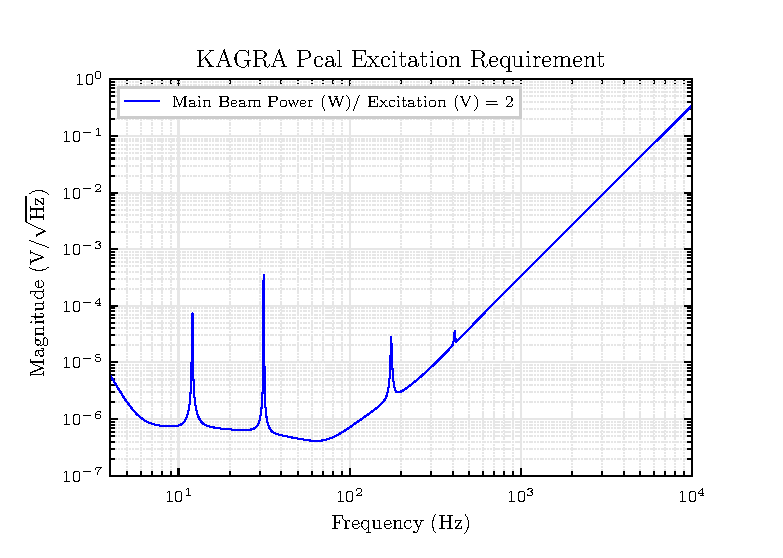
\includegraphics[width=.9\textwidth]{figure/DAC_requirement.eps}
\caption{Injection Channel Noise Requirement}\label{fig:DAC_noise_requirement}
\index{figures}
\end{figure}

\begin{align}
%\label{eq:}
   \Delta L(f) &< \frac{1}{10} \times (\text{KAGRA length sensitivity})\\
   \Delta L(f) =\frac{2 \Delta P(f) \cos(\theta)}{c} \frac{1}{M(2 \pi f)^2} &< \frac{1}{10} \Delta h(f) L
\end{align}








\section{Noise Source of Excitation channel}
\subsection{Quantization Noise of DAC}


The origin of quantization error is coming from the difference between desired analog output and quantized Digital to Analog Converter(DAC) output value. Roughly speaking, it shows like white noise spreading from DC to Nyquist frequency i.e. $Fs/2$.
The Root Mean Square value of quantization noise has the order of voltage difference corresponding to last digit or Least Significant Bit(LSB). In time domain, we can calculate standard deviation.
\begin{align}
%\label{eq:}
   \sigma_x = \sqrt{\frac{1}{12}} \delta x_{LSB}
\end{align}

For a 16-bit 64kHz DAC with output range between $\pm 10$Volts, 
\begin{align}
%\label{eq:}
    \sigma_x &= \sqrt{\frac{1}{12}} \delta x_{LSB} \\
             &= \sqrt{\frac{1}{12}} \frac{(+10)-(-10) \mathrm{Volts}}{2^{16}} \\
             &= 8.81 \times 10^{-5} \;\mathrm{Volts}
\end{align}

In frequency Domain, the quantization noise is distributed from DC to 32768Hz; therefore, we have ASD
\begin{align}
%\label{eq:}
    ASD &= \sqrt{PSD} \\
        &= \sqrt{ \frac{\sigma_x^2}{32768} } \\
        &= 8.81 \times 10^{-5} \sqrt{\frac{1}{32768}} \\
        &= 4.87 \times 10^{-7} \;\mathrm{Volts}/\sqrt{\mathrm{Hz}} 
\end{align}





\section{Noise Reduction through de-whitening filter}
Problem of 16kHz excitation channel 
Implementation of 64kHz Excitation channel in KAGRA digital system

Principle of Analog filter
Design of De-Whitening filter
Performance test
Transfer function measurement 
Noise requirement
Create Inverse De-Whitening filter






\chapter{Validation of Injection Channel}
Noise measurement
around 100Hz  the nose should below the IFO sensitivity
Transfer Function measurement
“above 1kHz” performance
time delay of excitation channel
(absolute timing measurement?)
Distortion of Scientific Signal
BBH
BNS post merger





\appendix % all chapters following will be labeled as appendices
\chapter{Implementation Details\label{ch:implementation}}

Appendices are just chapters, included after the $\backslash appendix$ command.

\section{Switching Formats}
When switching \texttt{printmode} on and off (see Section~\ref{sec:usage:options}), you may need to delete the output .aux files to get the document code to compile correctly. This is because the hyperref package is switched off for \texttt{printmode}, but this package inserts extra tags into the contents lines in the auxiliary files for PDF links, and these can cause errors when the package is not used.

\section{Long Tables}

Long tables span multiple pages. By default they are treated like body text, but we want them to be single spaced all the time. The class therefore defines a new command, $\backslash tablespacing$, that is placed before a long table to switch to single spacing when the rest of the document is in double spacing mode. Another command, $\backslash bodyspacing$, is placed after the long table to switch back to double spacing. Normal tables using \texttt{tabular} automatically use single spacing and do not require the extra commands.

When the documentclass is defined with the `singlespace' option, these commands are automatically adjusted to stay in single spacing after the long table.

Make sure there is always at least one blank line after the $\backslash bodyspacing$ command before the end of the file.

Some times long tables do not format correctly on the first pass. If the column widths are wrong, try running the \LaTeX compiler one or two extra times to allow it to better calculate the column widths.

If you want your long table to break pages at a specific point, you can insert the command $\backslash pagebreak[4]$, to tell \LaTeX that it really should put a page break there. $\backslash pagebreak[2]$ gives it a hint that this is a good place for a page break, if needed. If there's a row that really should not be broken across a page, use $\backslash \backslash *$, which will usually prevent a pagebreak. 

\section{Booktabs}
The booktabs package is included to print nicer tables. See the package documentation~\cite{fear2005booktabs} for more details and motivation. Generally, all vertical lines are removed from the tables for a better visual appearance (so don't put them in), and better spacing and line thicknesses are used for the horizontal rules. The rules are defined as $\backslash toprule$ at the top of the table, $\backslash midrule$ in between the heading and the body of the table (or between sections of the table), and $\backslash bottomrule$ at the end of the table. $\backslash cmidrule$ can be used with the appropriate options to have a rule that spans only certain columns of the table.

\section{Bibliography and Footnotes}

The bibliography and any footnotes can also be single spaced, even for the electronic copy. The template is already setup to do this.

Bibliography entries go in the .bib file. As usual, be sure to compile the \LaTeX code, then run BibTeX, and then run \LaTeX again.

To cite websites and other electronically accessed materials, you can use the `@electronic' type of BibTeX entry, and use the `howpublished' field to include the URL of the source material.

The formatting of bibliography entries will be done automatically. Usually the titles are changed to have only the first word capitalized. If you'd prefer to have your original formatting preserved, place the title in an extra set of curly braces, i.e., ``title = \{\{My title has an AcroNyM that should stay unchanged\}\},''.

\section{Figures and Tables}
The captions of figures and tables take an optional parameter in square brackets, specifying the caption text to be used in the Table of Contents. The regular caption in curly braces is used for the table itself.

Generally captions for tables are placed above the table, while captions for figures are placed below the figure.




\chapter{Printing and Binding\label{ch:printing}}

\section{Printing}

For the library copies of your dissertation, you must use archival quality printing and binding. This means acid-free paper, containing at least 25\% cotton fiber. Triangle Repocenter on Nassau Street in Princeton offers both 25\% cotton paper and 100\% cotton paper. Most people choose the 25\% cotton paper, and this is generally recommended by the binders. The 100\% copy paper is somewhat thicker and the extra expense is unnecessary. 

Triangle offers online submission of your printing and binding order at: \url{http://triangleprinceton.com/collegiatebinding/thesis/}. If you request binding from them, they will deliver the paper copies to Smith-Shattuck Bookbinding for you and allow you to pick up the completed copies at their store on Nassau Street. The whole process takes 2-3 business days, but check with them in advance during the busy thesis-printing season in April and May. 

Currently, your printed and bound dissertation copies can be single spaced. Only the electronic copy submitted to ProQuest must be double spaced. All copies must be printed single-sided, with specific margins. 

\section{Binding}

An archival-quality sewn binding is required for the library copies of your dissertation. Smith-Shattuck Bookbinding is highly recommended, and is used by most students. Triangle Repocenter will send your copies there for you, greatly simplifying the process, but you can call Smith-Shattuck with special requests. 

The ``library standard'' sewn binding is sufficient for the copies to be sent to Mudd Library. It uses a black buckram cloth cover, which is the most popular option. For extra copies for yourself and your family members, you can choose ``buckram roundback binding'', which adds decorative lines on the spine, and printing of the title and author on the front cover. For a small additional fee, you can include the Princeton University shield on the front cover and a ribbon bookmark. Leather covers are also available. See Smith-Shattuck's website for more details at: \url{http://www.thesisbookbinding.com/}. 


% Make the bibliography single spaced
\singlespacing
\bibliographystyle{plain}

% add the Bibliography to the Table of Contents
\cleardoublepage
\ifdefined\phantomsection
  \phantomsection  % makes hyperref recognize this section properly for pdf link
\else
\fi
\addcontentsline{toc}{chapter}{Bibliography}

% include your .bib file
\bibliography{thesis}

\end{document}

